\documentclass[12pt]{article}
\usepackage[margin=1in]{geometry}
\usepackage{graphicx}
\usepackage{amsmath}
\setlength{\parindent}{0pt}

\begin{document}

\title{Diffusion for Imitation Learning}
\author{Devesh}
\date{\today}

\maketitle

\begin{abstract}
My notes for diffusion for imitation learning.
\end{abstract}

\section{Neural Ordinary Differential Equations}
\textbf{Scalar Loss Function:} $L(z(t_1)) = L\left(z(t_0) + \int_{t_0}^{t_1} f(z(t), t, \theta) \, dt\right) = L(\mathrm{ODESolve}(z(t_0), f, t_0, t_1, \theta))$

\textbf{State Dynamics:} $\frac{dz(t)}{dt} = f(z(t), t, \theta)$

\textbf{Lagrangian:} $L(u, p, z, \lambda) = J(u, p) + \int_{t_0}^{t_1} a(t)^\top \left( \frac{dz(t)}{dt} - f(z(t), u, p) \right) \, dt$, for some cost J

\textbf{Adjoint Dynamics:} \(a(t_N) = \frac{\partial L}{\partial z(t_N)}\), $\frac{da(t)}{dt} = -a(t)^\top \frac{\partial f(z(t), t, \theta)}{\partial z(t)}$

\textbf{Parameter Gradient:} $\frac{\partial L}{\partial \theta} = -\int_{t_0}^{t_N} a(t)^\top \frac{\partial f(z(t), t, \theta)}{\partial \theta} \, dt$

\subsection{Comparison with Resnets}
Resnets are a special case of Neural ODEs, where euler integration is used to model dynamical systems $x_{t+1} = x_{t} + f(x_{t}, u)$. Numerical integration requires to store the states of the system in memory and doesnt perform well for long sequences. 
Resnets also require data to be regularly spaced in time which is often constraining. Neural ODEs on the other hand, only require to store the initial state and the parameters of the ODE, and can be trained using reverse-mode differentiation.

\subsection{Reverse-Mode Differentiation or Backpropagation} 
Neural ODEs model the dynamics of the continuous function directly. We have $\{t_{0} ... t_{N}\}$ points to equally spaced points to discretize calculation of the Neural ODE. Data can be irregulary spaced and can occur anywhere in this interval.
At $t_{N}$, \(a(t_N)= \frac{\partial L}{\partial z(t_N)}\) is calculated. Then using $\frac{da(t)}{dt} = -a(t)^\top \frac{\partial f(z(t), t, \theta)}{\partial z(t)}$ the adjoint state is propagated back in time.
To calculate the adjoint state, z(t) is required but unlike Resnets, $z(t)$ is not stored but is calculated by solving the ODE $\frac{dz(t)}{dt} = f(z(t), t, \theta)$ backwards in time until we reach a data point $z(t_i)$.
At the data point, $a(t_{i})$ is calculated similarly to $a(T_{N})$. There is a discrepancy (shown in figure 2) between the propagated adjoint dynamics and the dynamics at this data point, which is minimzed to get continuous adjoint state dynamics. 
When we have the entire adjoint dynamics, we can calculate the gradient of the parameters $\theta$ using $\frac{\partial L}{\partial \theta} = -\int_{t_0}^{t_N} a(t)^\top \frac{\partial f(z(t), t, \theta)}{\partial \theta} \, dt$. 

\begin{figure}[ht]
    \centering
    \begin{minipage}{0.45\textwidth}
        \centering
        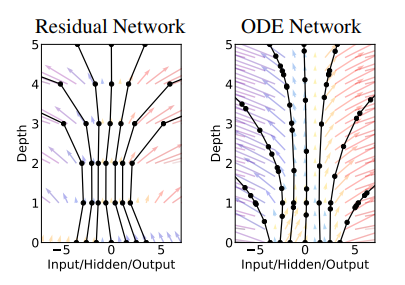
\includegraphics[width=\textwidth]{1.png}
        \caption{Resnets vs Neural ODEs}
        \label{fig:1}
    \end{minipage}\hfill
    \begin{minipage}{0.45\textwidth}
        \centering
        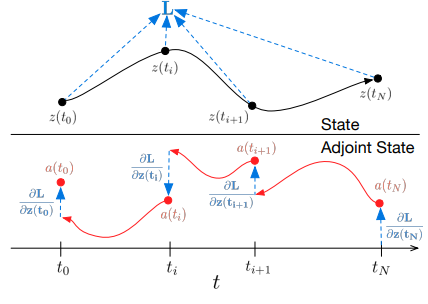
\includegraphics[width=\textwidth]{2.png}
        \caption{Adjoint and State Dynamics, Reverse-Mode Differentiation}
        \label{fig:2}
    \end{minipage}
\end{figure}

\subsection{Normalizing Flows}
Normalizing flows use a sequence of transformations \(f_1, f_2, \ldots, f_K\), where each transformation is invertible and differentiable, to map samples from a simple base distribution \(p_X(x)\) to a target distribution \(p_Z(z)\) (e.g., standard Gaussian).
In Normalizing Flows, the transformation $f$ is a learned bijective function:
\[
    z_1 = f(z_0) \Rightarrow \log p(z_1) = \log p(z_0) - \log \left| \det \frac{\partial f}{\partial z_0} \right|
\]
Calculating the determinant is computationally expensive. Instead, continuous normalizinf flows are used. Planar Flow:
\[
    f(z(t+1)) = z(t) + uh(w^\top z(t) + b)
\]
CNFs generalize normalizing flows by moving from discrete transformations (layers) to continuous transformations using differential equations. 
A CNF is defined by a time-dependent differential equation:
\[
\frac{dz(t)}{dt} = f(z(t), t),
\]
where \( f \) is a neural network parameterized by learnable weights.

The probability density evolves according to the instantaneous change of variables theorem:
\[
\frac{\partial \log p(z(t))}{\partial t} = -\mathrm{tr}\left(\frac{\partial f}{\partial z(t)}\right),
\]
where \(\mathrm{tr}(\cdot)\) is the trace of the Jacobian matrix \(\frac{\partial f}{\partial z(t)}\). 
In CNFs, the trace of the Jacobian \(\mathrm{tr}\left(\frac{\partial f}{\partial z}\right)\) allows wide layers (many hidden units) to be evaluated efficiently, scaling linearly with the number of hidden units \(M\).
If the dynamics are defined as a sum of multiple functions:
\[
\frac{dz(t)}{dt} = \sum_{n=1}^{M} f_n(z(t)),
\]
the log-density evolves as:
\[
\frac{\partial \log p(z(t))}{\partial t} = \sum_{n=1}^{M} \mathrm{tr}\left(\frac{\partial f_n}{\partial z}\right).
\]
This decomposition makes the model highly expressive while keeping computations efficient.
The dynamics \(f(z(t), t)\) can depend explicitly on time \(t\), allowing the transformation to vary continuously over time.
Gating mechanisms \(\sigma_n(t) \in (0, 1)\) control when specific dynamics \(f_n(z)\) are active:
\[
\frac{dz}{dt} = \sum_{n} \sigma_n(t) f_n(z).
\]
This makes the model more interpretable and adaptable to the structure of the data. In both NFs and CNFs, hidden units correspond to neurons (i.e., individual computational units in the parameterizing neural network).
The layers in discrete NFs correspond to discrete transformations, whereas in CNFs, the transformation is continuous, so there are no explicit "layers"—only a time-evolving flow parameterized by the hidden units.
\end{document}